% Gemini theme
% https://github.com/anishathalye/gemini

\documentclass[final]{beamer}

% ====================
% Packages
% ====================

\usepackage[T1]{fontenc}
\usepackage{lmodern}
\usepackage[size=custom,width=120,height=72,scale=1.0]{beamerposter}
\usetheme{gemini}
\usecolortheme{gemini}
\usepackage{graphicx}
\usepackage{booktabs}
\usepackage{tikz}
\usepackage{pgfplots}

\DeclareMathOperator*{\argmax}{\arg\max}

% ====================
% Lengths
% ====================

% If you have N columns, choose \sepwidth and \colwidth such that
% (N+1)*\sepwidth + N*\colwidth = \paperwidth
\newlength{\sepwidth}
\newlength{\colwidth}
\setlength{\sepwidth}{0.025\paperwidth}
\setlength{\colwidth}{0.3\paperwidth}

\newcommand{\separatorcolumn}{\begin{column}{\sepwidth}\end{column}}

% ====================
% Title
% ====================

\title{BCFW and Dual extragradient, two complementary approaches to structured optimization}
\author{William St-Arnaud\inst{1} \and Fr\'ed\'eric Boileau \inst{1} \and Elyes Lamouchi\inst{1}}

\institute[shortinst]{\inst{1} Universit\'e de Montr\'eal}

% ====================
% Body
% ====================

\begin{document}

\begin{frame}[t]
\begin{columns}[t]
\separatorcolumn

\begin{column}{\colwidth}

  \begin{block}{}

    \begin{figure}
      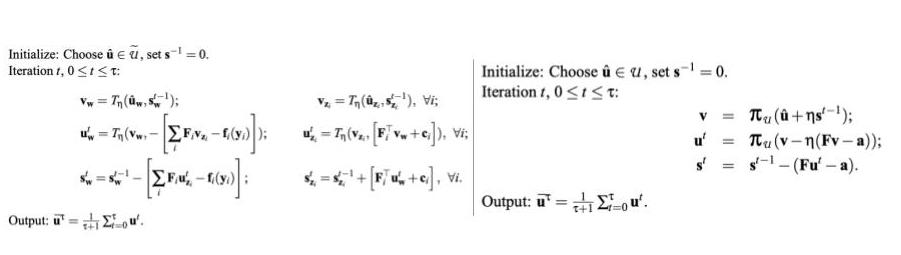
\includegraphics{img/extra_grad.jpg}
      \caption{Dual extragradient algorithm with Euclidean projections and Bregman projections}
      \label{extragrad}
    \end{figure}
  \end{block}


  \begin{block}{Dual extragradiant alogrithm}
    The dual extragradiant takes advantage of the min-max formulation of the problem. Instead of dualizing the max oracle and peforming FW or projected gradient descent, we could try alternating between updates for the max and min (can see them as opponents).
    However this can lead to oscillation. 
    A better way would be to combine the two vectors we update alternatively into one and then perform two gradient udpates. The
    first one is called a ``look-ahead'' step. This step consists in starting from a point inside the constraint set and moving away
    from it  by a little amount and then projecting back to the constraint set. The second step consists in performing the gradient
    udpate using the look-ahed point. Then, we update the trajectory completed so far so that the next iteration can perform a  look-ahead
    step using that starting point.
    \begin{itemize}
      \item The dual extragradient algorithm takes advantage of the min-max (saddle-point) formulation. No need to find the dual of
	one of the objectives.
      \item We can use this formulation on many more problems for which we do not have a parameter space defined
	by linear and convex quadratic constraints which are necessary for using commercial solvers.
    \end{itemize}

    The most intuitive type of projection that can be used is the Euclidean projection.
    However, for some problems these are expensive to compute (e.g. think cuts or matching problems)
    The method that we present introduces the concept of Bregman projections.
    The Bregman projection comes from the Bregman divergence. The Bregman divergene between $u$ and $u'$ for a strongly convex function 
    $h$ is simply an upper bound to the squared  norm of $u' - u$ :
    \begin{equation*}
      d(u', u) = h(u') - h(u) - \nabla h(u)^T (u' - u) \geq \lVert u' - u \rVert^2
    \end{equation*}
    The Bregman projection is then the following operator:
    \begin{equation*}
      T_{\eta}(u,s) = \argmax_{u' \in \mathcal{U}} \left[ s^T (u' - u) - \frac{1}{\eta} d(u', u)\right]
      \end{equation*}
    \begin{itemize}
      \item Bregman projections are easier to derive a projection for some problems where Euclidean projections are hard (e.g. matchings)
      \item We only need a strongly convex function for the norm on the combined parameters (i.e. $u = (w,z)$).
    \end{itemize}
  \end{block}
  
  \begin{block}{References}

    \nocite{*}
    \footnotesize{\bibliographystyle{plain}\bibliography{poster}}

  \end{block}

\end{column}

\separatorcolumn

\begin{column}{\colwidth}

  \begin{alertblock}{Face Expression Comparison dataset (FEC)}
    In our experiments, we used the FEC dataset. It consists of 3-tuples of face images. In each tuple, a person has labeled the 
    the two images that likely depict the same emotion. The emotion labels of each image were picked from another dataset. The 3-tuples
    are labeled as ONE-CLASS, TWO-CLASS, or THREE-CLASS. This simply tells us how many emotions are shown in the three images. The data
    was split into a training set and a test set.

    We extracted all images and resized them to $32 \times 32$ images to have a fixed dimension for the features. The feature vectors
    were then simply a concatenation of two flattened images. As there were three labels possible (e.g. 1-2, 1-3, and 2-3), we had three
    possible features per 3-tuple. The size of the feature vectors was thus $32 \times 32 \times 2 = 2048$

    \begin{figure}
      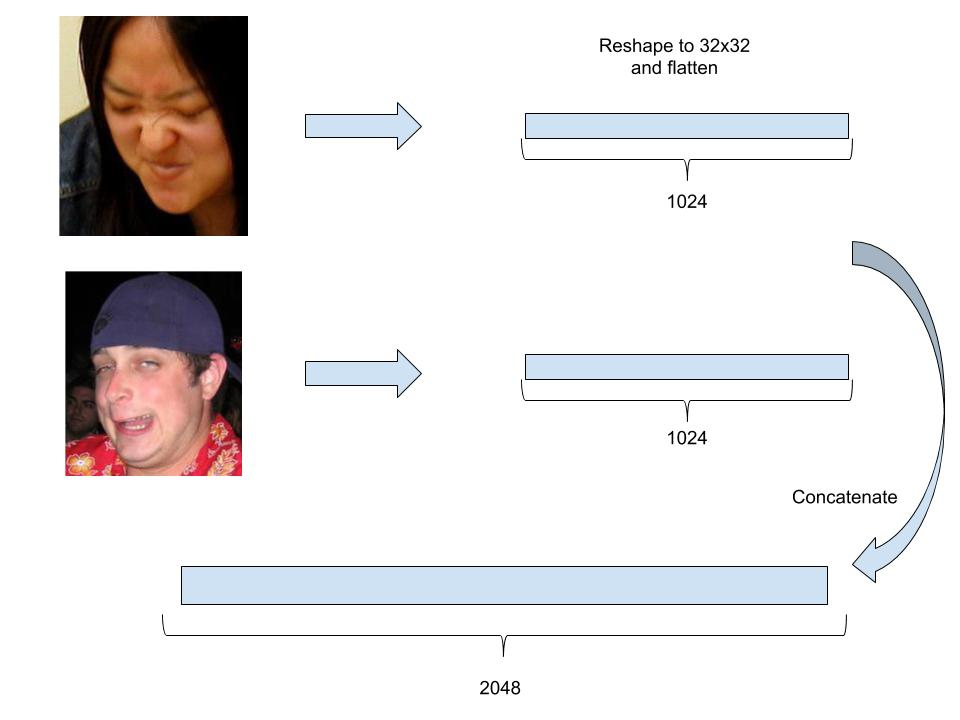
\includegraphics[scale=0.75]{img/fec_poster.jpg}
      \caption{How the feature vectors are extracted from two images}
      \label{feat_vec}
    \end{figure}
  \end{alertblock}

    \begin{figure}
     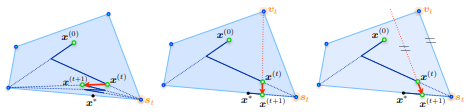
\includegraphics[width=\linewidth]{img/fig2.png}
     \caption{(left) The FW algorithm zig-zags when the solution $x$ lies on the boundary. (middle) Adding the possibility of an away step attenuates this problem. (right) As an alternative, a pairwise FW step.}
    \label{fig:Away steps}
   \end{figure}
    
    \begin{table}
      \centering
      \begin{tabular}{l r r r c}
        \toprule
        \textbf{Extragradient |} & \textbf{Frank-Wolfe |} & \textbf{Block coordinate FW |} & \textbf{Away-steps FW |} & \textbf{Randomized AFW}\\
        \midrule
        Sublinear & Sublinear & Sublinear & Linear & Linear\\
        exercice to the reader?? & $\mathcal{O}(Kn)$ & $\mathcal{O}(n)$ & $\mathcal{O}(Kn)$ & $\mathcal{O}(K\eta n)$\\
        \bottomrule
      \end{tabular}
      \caption{Convergence rates}
    \end{table}   
   
   
\end{column}


\separatorcolumn

\begin{column}{\colwidth}

  \begin{block}{Frank-Wolfe variants in different contexts}
    Consider the problem of minimizing a convex objective function $f$ over the convex hull of its domain $\mathcal{M}= conv(\mathcal{A})$.\\
    By minimizing the first-order approximation of the objective function, the Frank-Wolfe algorithms takes a convex combination of the immediate iterate with the previous one. Suppose having access to an efficient \textit{\textbf{L}inear \textbf{M}inimization \textbf{O}racle},
    \begin{equation*}
    \begin{aligned}
        &LMO_{\mathcal{A}}(\nabla f(x_{t}))\in \textit{argmin}_{s\in\mathcal{A}}\langle s, \nabla f(x_{t})\rangle
    \end{aligned}    
    \end{equation*}
    For the $t^{th}$ iteration, we call $s_{t}= LMO_{\mathcal{A}}(\nabla f(x_{t}))$, an "atom".\\
    Starting with an active set of an initial feasible point $S^{(t=0)}= \{x_{0}\}$, at each iteration the Frank-Wolfe algorithm adds an "atom" , to $S^{(t)}$ by taking a convex combination of $s_{t}$ with its elements. Just like subgradient methods, this algorithm converges at a sublinear rate.\\
    However, in a structured SVM setting, with $LMO_{\mathcal{A}}$ being equivalent to maximizing the hinge loss on $\mathcal{Y}_{i}$ where $i\in\{1..n\}$\quad batch FW requires $n$ calls to the max oracle each iteration. Which can make subgradient methods a more practical alternative.\\
    Depending on the domain of the objective we have 2 alternatives:
    \begin{itemize}
      \item When the domain has the structure of a Cartesian product $\mathcal{M}=\mathcal{M}^{(1)}\times...\times\mathcal{M}^{(n)}$, and the objective is convex, we can perform update steps one block at a time while still converging to a global minimum.\\
     While this looks like coordinate descent, in \textit{Block coordinate Frank-Wolfe}, we choose the coordinate at random.\\
     Hence BCFW is $n$ times faster than the classical F-W, while still keeping a sublinear convergence rate.
      \item When the domain is non-separable (e.g. $l_{1}$ constrained optimization), at each iteration, we call the $LMO$ on an $\eta\in(0,1]$\quad subsample of $\mathcal{A}$.\\
      By doing this, each iteration costs $\eta$ times cheaper than classical FW, while keeping a sublinear convergence rate
    \end{itemize}
  \end{block}
    \begin{block}{Speeding up convergence}
    When the minimizer of the objective function lies at the boundary of the domain, the F-W algorithm starts to zig-zag around the descent direction as can be seen in figure 3.
    \begin{itemize}
    \item  \textbf{Away-steps Frank-Wolfe: }Due to the strong dependency of the immediate iterate on previously accumulated atoms in the active set, as it approaches to boundary, FW starts going in non-descent directions.\\
    To address this issue an improved variant of F-W named \textit{Away-steps Frank-Wolfe} adds the possibility of moving away from a non-descent direction by removing a fraction of a maximizer of the $LMO_{\mathcal{S}_{t}}$.\\
    While this slows down each iteration it should be noted that the added step is easier than $LMO_{\mathcal{A}}$ given that we maximize over a subset of $\mathcal{A}$.\\ The resulting variant converges linearly, and as the algorithm progresses in a fewer number of iterations in the descent direction, it is much faster than the original F-W.
    \item \textbf{Randomized Away-steps Frank-Wolfe}
    By subsampling a $\eta\in(0,1]$ portion of the domain $\mathcal{A}$ in the $LMO$ and adding an away step at each iteration, the Randomized Away-steps Frank-Wolfe (RAWF) combines the best of both words.\\
    While being applicable in non sparable domains, unlike BCFW we have a linear convergence rate and cheaper oracle calls than that of the original F-W.
    \end{itemize}
  \end{block}

\end{column}

\separatorcolumn
\end{columns}
\end{frame}

\end{document}
